\section{Design}

Figure \ref{pic:db_schema1} shows the database schema for the first
pin tool, that records all memory operations. The schema consists of
the following tables:
\begin{description}
  \item[Images] Tracks information about which images
    (i.e. executables and dynamic libraries) are used by the
    program). The table records the name (\texttt{ImgName}) of the
    image and an associated, unique numerical identifier
    (\texttt{Id}).
  \item[Calls] Records all methods calls performed during
    execution. An entry consists of the simulation time
    (\texttt{VLCK}) the event occurred, the memory base address
    (\texttt{Method}) of the method and the action (\texttt{Enter}),
    i.e. whether the program entered or left the method.
  \item[Methods] Contains all available methods during the execution
    of the program. An entry of this table consists of the Method name
    (\texttt{MethName}), the id (\texttt{ImgId}) of the image within
    which the method is located, the base address (\texttt{MethStart})
    at which the method is located in memory and the address of the
    last method instruction (\texttt{MethEnd}).
  \item[MemoryAccesses] Records all occurred memory accesses. If an
    instruction has more than one memory access (e.g., instruction and
    data access) then multiple entries are generated. An entry
    consists of the simulation time (\texttt{VLCK}) the event
    occurred, The memory address that is accesses
    (\texttt{MemAddress}), the address of the instruction that
    triggered the event (\texttt{InstrAddress}), an numerical value
    (\texttt{ThreadId}) specifying in which thread the event occurred
    and field identifying (\texttt{Write}) whether the operation was a
    read or write.
  \item[Frees] This table records all executed \texttt{free} calls. An
    entry in this table consists of the simulation time
    (\texttt{VLCK}) the call occurred and the base address
    (\texttt{Address}) of the buffer.
  \item[Mallocs] This table records all memory allocations via
    \texttt{malloc}. An entry in this table consists of the simulation
    time (\texttt{VLCK}) the call occurred, the size of the allocated
    buffer (\texttt{Size}) and the base address (\texttt{Address}) of
    the buffer.
\end{description}

\begin{figure}
  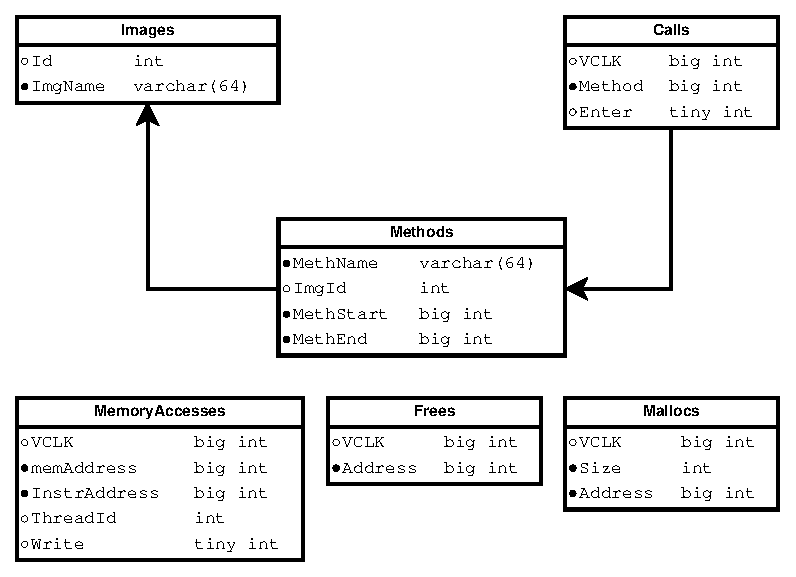
\includegraphics[width=\columnwidth]{database_schema1}
  \caption{Database Schema Pin-Tool1}
  \label{pic:db_schema1}
\end{figure}


\begin{figure}
  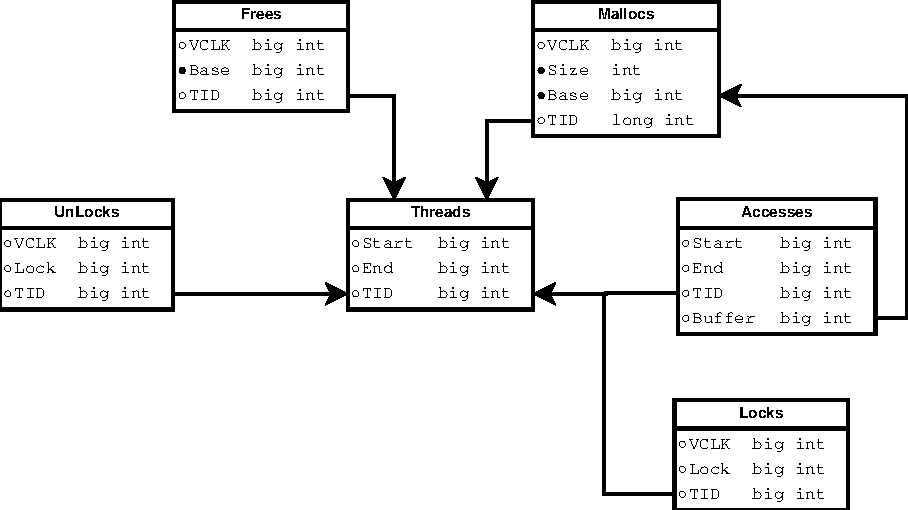
\includegraphics[width=\columnwidth]{database_schema2}
  \caption{Database Schema Pin-Tool2}
  \label{pic:db_schema2}
\end{figure}
